% This LaTeX was auto-generated from MATLAB code.
% To make changes, update the MATLAB code and export to LaTeX again.

\documentclass{article}

\usepackage[utf8]{inputenc}
\usepackage[T1]{fontenc}
\usepackage{lmodern}
\usepackage{graphicx}
\usepackage{color}
\usepackage{listings}
\usepackage{hyperref}
\usepackage{amsmath}
\usepackage{amsfonts}
\usepackage{epstopdf}
\usepackage{matlab}

\sloppy
\epstopdfsetup{outdir=./}
\graphicspath{ {./hw2_exe_images/} }

\begin{document}
\matlabtitle{Empirical Methods HW2}
\matlabtitle{Carlos Rangel}

\begin{matlabcode}
% Declare Parameters
% Make them global so that they can be read by the functions

% Qualities of each product
global va;
global vb;
\end{matlabcode}


\matlabheading{Question 1:}

\begin{par}
\begin{flushleft}
Consider the following parameterization: va=vb=2. What is the demand for each option if pa=pb=1?
\end{flushleft}
\end{par}

\begin{matlabcode}
% Define quality parameters
va=2;
vb=2;

% Define Price vector
p=[1;1];

% Compute and Display Demands

% Demand for product A
da=DA(p)
\end{matlabcode}
\begin{matlaboutput}
da = 0.4223
\end{matlaboutput}
\begin{matlabcode}

% Demand for product B
db=DB(p)
\end{matlabcode}
\begin{matlaboutput}
db = 0.4223
\end{matlaboutput}
\begin{matlabcode}

% Demand for the outside product
d0=D0(p)
\end{matlabcode}
\begin{matlaboutput}
d0 = 0.1554
\end{matlaboutput}


\matlabheading{Question 2.}

\begin{par}
\begin{flushleft}
Given the above parameterizations for values, use Broyden's method to solve for the Nash pricing equilibrium. (Hint: There is a unique equilibrium.) Report the staring value and convergence criteria ( if it converges)
\end{flushleft}
\end{par}

\begin{matlabcode}
% Starting value
x0=[1;1];

% Solve the System of Nonlinear Equations and time it
% Use the Broyden Function from the Miranda-Fackler CompEcon Toolbox (Must be added to path)
% This Broyden function uses Convergence Criteria: sqrt(machine epsilon)
tic
prices_sol=broyden('focs', x0)
\end{matlabcode}
\begin{matlaboutput}
prices_sol = 2x1    
    1.5989
    1.5989

\end{matlaboutput}
\begin{matlabcode}
toc
\end{matlabcode}
\begin{matlaboutput}
Elapsed time is 0.017307 seconds.
\end{matlaboutput}


\matlabheading{Question 3.}

\begin{par}
\begin{flushleft}
Now use a Gauss-Seidel Method (using the secant method for each subiteration) to solve for the pricing equilibrium. Which method is faster?
\end{flushleft}
\end{par}

\begin{matlabcode}
% Start with initial guesses
p0=[1;1];
p1=[2;2];

% Set tolerance Criteria
tol=sqrt(eps);

% Set Maximum Iterations for the outer iterations 
maxit=1000;

% Maximum Subiterations
maxsubit=1000;

% The Gauss Seidel method (using the secant condition for each subiteration) is defined in the function nonlin_gs
% it takes as arguments two initial guesses, the maximum number of iterations and subiterations
tic
sols=nonlin_gs(p0, p1, tol, maxit, maxsubit)
\end{matlabcode}
\begin{matlaboutput}
sols = 2x1    
    1.5989
    1.5989

\end{matlaboutput}
\begin{matlabcode}
toc
\end{matlabcode}
\begin{matlaboutput}
Elapsed time is 0.015983 seconds.
\end{matlaboutput}

\begin{par}
\begin{flushleft}
Both methods take roughly the same amount of time. However, Miranda-Feckler's Broyden method also performs line search, which may be taking up additional time. So it could be that without it, Broyden's method may actually work faster. Broyden's method could work faster because of the fact that it incorporates information from all of the nonlinear equations(through the Jacobian) at a given iterate in determining the direction it takes for the next iterate. For the method proposed in Question 3,however, we only work with one nonlinear equation at a time.
\end{flushleft}
\end{par}

\vspace{1em}


\matlabheading{Question 4.}

\begin{par}
\begin{flushleft}
Lastly, use the following update rule to solve for the equilibrium:
\end{flushleft}
\end{par}

\begin{par}
\begin{flushleft}
p\_t+1 = 1/(1-D(p\_t))
\end{flushleft}
\end{par}

\begin{par}
\begin{flushleft}
Does this converge? Is it faster or slower than the other two methods?
\end{flushleft}
\end{par}

\begin{matlabcode}
% Tolerance levels (if the difference between two succesive iterates is
% less than tol, we have converged)
tol=sqrt(eps);

% Stop if we have exceeded maxits iterations
maxits=1000;

% Initial Guess
p0=[1;1];

% Solve the nonlinear system of equations using the proposed update rule
% and time it
tic
psols=q3_update(p0, tol, maxits)
\end{matlabcode}
\begin{matlaboutput}
psols = 2x1    
    1.5989
    1.5989

\end{matlaboutput}
\begin{matlabcode}
toc
\end{matlabcode}
\begin{matlaboutput}
Elapsed time is 0.041520 seconds.
\end{matlaboutput}

\begin{par}
\begin{flushleft}
This method is somewhat slower than the other two, but around the same order of magnitude.
\end{flushleft}
\end{par}


\matlabheading{Question 5.}

\begin{par}
\begin{flushleft}
Solve the pricing equlibrium (using your preferred method) for va=2 and vb=0:0.2:3. On the same graph, plot Pa and Pb as a function of the vector of vb.
\end{flushleft}
\end{par}

\begin{matlabcode}
vb_vector = 0:0.2:3;

n_vb=length(vb_vector);

pa_vector=zeros(n_vb,1);
pb_vector=zeros(n_vb,1);

x0=[1;1];
for i=1:n_vb
 vb = vb_vector(i);
 prices_sol = broyden('focs', x0);
 pa_vector(i) = prices_sol(1);
 pb_vector(i) = prices_sol(2);
 x0=prices_sol;
end


plot(vb_vector, pa_vector, vb_vector, pb_vector)
legend('Pa','Pb')
xlabel('Vb')
ylabel('Prices')
\end{matlabcode}
\begin{center}
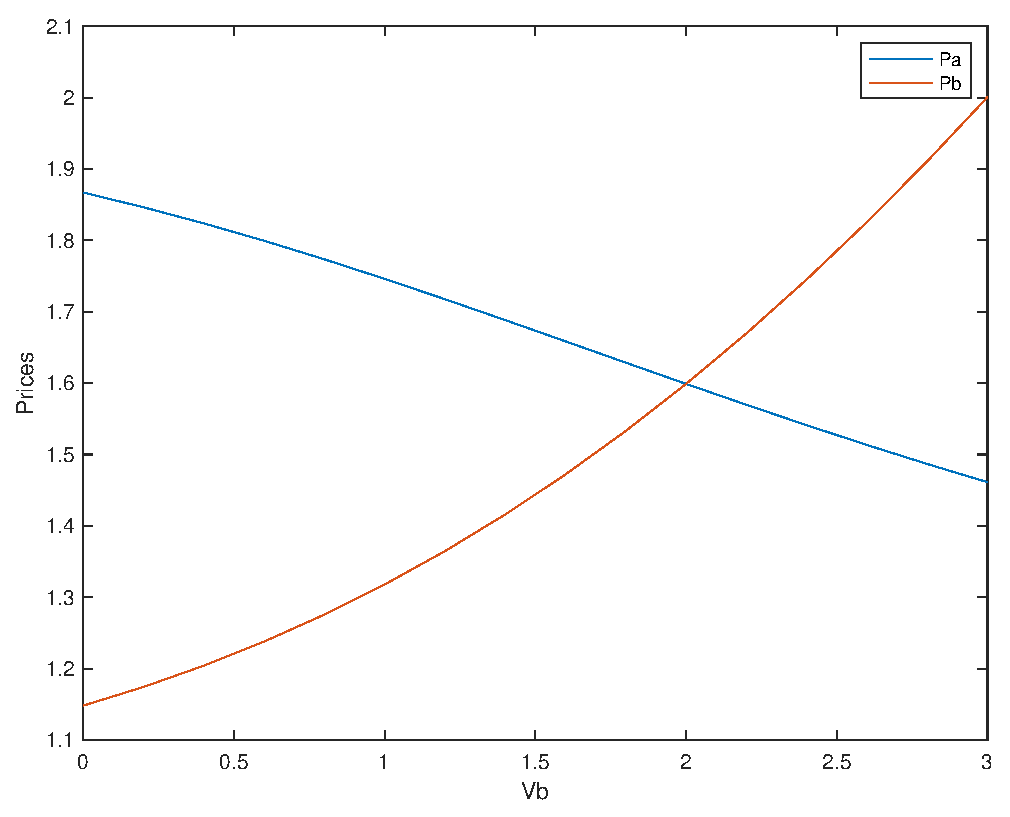
\includegraphics[width=\maxwidth{56.196688409433015em}]{figure_0}
\end{center}
\begin{matlabcode}


\end{matlabcode}

\end{document}
